\documentclass[12pt]{article}

\usepackage{graphicx}
\usepackage{paralist}
\usepackage{listings}
\usepackage{booktabs}
\usepackage{hyperref}
\usepackage{subfig}
\usepackage{float}

\oddsidemargin 0mm
\evensidemargin 0mm
\textwidth 160mm
\textheight 200mm

\pagestyle {plain}
\pagenumbering{arabic}

\newcounter{stepnum}

\title{CS/SE 2XB3 Lab 4 Report\\Enrolled in CSL02}
\author{
  Wang, Mingzhe\\400316660\\
  \texttt{wangm235@mcmaster.ca}
  \and
  Li, Xing\\400292346\\
  \texttt{li64@mcmaster.ca}
  \and
  Moon, Hyosik\\400295620\\
  \texttt{moonh8@mcmaster.ca}
  }
\date{\today}

\begin{document}

\maketitle

\tableofcontents


\section{Bottom-up}
We implement a helper function merge\_bottom(L, start, mid, end) to merge the sub-array L[start:mid] and L[mid: end]. We follow the python convention to include the left end and exclude the right end.

~\newline\noindent No recursion are used. We use only while loop and for loop. To deal with the issue that the list length may not be the power of 2, we use min() function to choose the minimum element between end index and n. We also compare middle index and n. If middle index is already greater than n, no bottom-up sort is needed.

~\newline\noindent To compare the bottom-up implementation to the original top-down algorithm in "lab4.py," we run both algorithm for 5 times and take the average run time as the base to compare. Then we run both algorithm with different lengths of list from 100 to 10,000, with a step of 100. There is convincing improvement on the run time with an average speed-up of 19\%.

~\newline\noindent As the merge part is the same in both algorithm, we guess that the difference may come from the lower space complexity in the bottom-up algorithm. The additional space required starts from 1 and doubles after each round of merge. Therefore, the average additional space usage is only $(\sum_{i=0}^{log_2 n} 2^i)/log_2 n \approx 2n/log_2 n$. In comparison, the merge sort space complexity is O(n). Less space requirement means less memory access, and this can result in the better performance in our case.

\begin{figure}[hbt!]
    \centering
    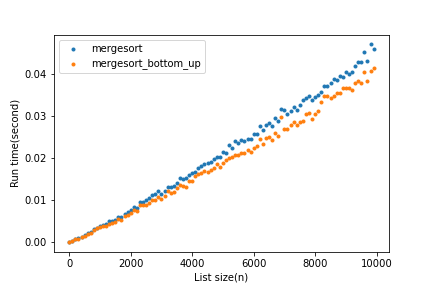
\includegraphics[width=0.5\textwidth]{Figures/mergesort_vs_mergesort_bottom_up.png}
    \caption{Bottom\_up vs Top\_down}
     \label{Figure: bottom_up}
\end{figure}

\section{Three-Way Mergesort}
\subsection{Prediction Before the Experiment}
Before starting testing \verb|mergesort_three| and \verb|merge_three|, we predict that \verb|mergesort_three| will perform no better or worse than \verb|mergesort|. The reason is that we can define a recurrence $T(n) = 3 * T(n/3) + O(n)$ for calculating the time complexity of \verb|merge_three|. By master theorem, the time complexity of \verb|merge_three| is $T(n) = O(n \log_3 n) = O(n \log n)$, which is the same as the time complexity of \verb|mergesort| $T(n) = O(n \log n)$.
\subsection{Compare the performance}
For comparing the performance of \verb|mergesort_three| and \verb|mergesort|, our testing method is consistent with the previous. Specifically, the list size $n$ is from $0$ to $20000$ with an interval $200$, and for each $n$, we run the test 5 times to decrease the noise from other factors. 

~\newline\noindent Our observation is that in average \verb|mergesort_three| is $16.28\% $ faster than \verb|mergesort|. In addition, we observe that  \verb|mergesort_three| is relatively more faster than  \verb|mergesort| when the list size is around $15000 \-- 20000$. The test result is showed in Figure \ref{Figure: mergesort_three}.

\begin{figure}[h!]
\centering
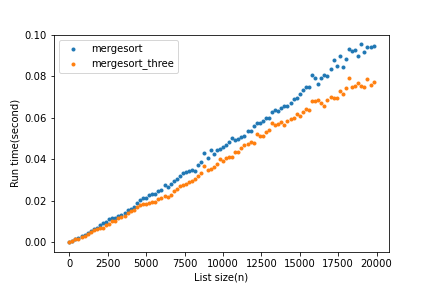
\includegraphics[width=0.5\textwidth,height=\textheight,keepaspectratio]{Figures/mergesort_vs_mergesort_three.png}
\caption{Mergesort vs Mergesort\_three}
\label{Figure: mergesort_three}
\end{figure}

\subsection{Result Explanation}
The experiment result shows that our prediction is wrong \--- \verb|mergesort_three| actually performs better than \verb|mergesort|. To explain this observation, we analyze these two algorithms, some of our perspectives are as the following:

~\newline\noindent Because the experiment result is the average time complexity, we cannot simply use Big-O notation to predict it. The actually running time of \verb|mergesort_three| should meet this recurrence $T(n) = 3 * T(n/3) + T'(n) = T'(n) \log_3 n$, where $ T'(n)$ is the actual time complexity of \verb|merge_three|. 

~\newline\noindent We assume that for each recursive call of \verb|merge_three|, the time consumed at the beginning (i.e. things like \verb|l = len(L) // 3|) can be omitted because they are not corresponding to list size. In addition, we assume all operations need constant time $t$.

~\newline\noindent Then, in our implementation of \verb|merge_three|, for each position of the merged list consisting of three subarrays, in the worst case, it needs 4 comparisons (i.e. \verb|i >= len(left)| or \verb|left[i] <= right[k]|), 1 \verb|append| (i.e. \verb|L.append(left[i])|), and 1 increment (i.e. \verb|i += 1|).  Based on this, the actual running time \verb|mergesort_three| needs is $6n \log_3 n = \frac{6}{\ln 3} n \ln n$. Similarly, because in the worst case there are 3 comparisons, 1 \verb|append| and 1  increment in \verb|mergesort|, the actual running time of \verb|mergesort| is $5n \log_2 n = \frac{5}{\ln 2} n \ln n$. Therefore, due to the fact that $\frac{6}{\ln 3} \approx 5.46 < 7.21 \approx \frac{5}{\ln 2}$, the actual running time of \verb|merge_three| should be faster than that of \verb|merge|, which verifies our observation.

\subsection{Another Consideration}
We have also noticed that the professor's version of \verb|mergesort| is not the "traditional" version of \verb|mergesort|. Its running time is not optimal because in the \verb|merge| method this version of implementation performs redundant comparisons when one of the subarray being merged is exhausted. And if we improve the professor's version of \verb|mergesort| to the real "traditional" version of \verb|mergesort|, the performance of \verb|mergesort| (improved prof's version) and \verb|merge_three| can be relatively similar as showed in Figure \ref{Figure: traditional_mergesort}.

\begin{figure}[h!]
\centering
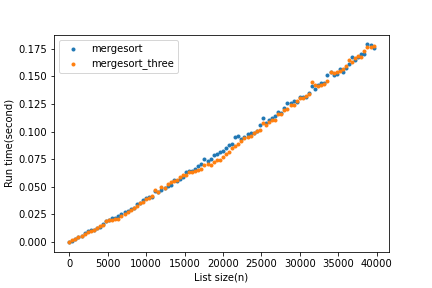
\includegraphics[width=0.5\textwidth,height=\textheight,keepaspectratio]{Figures/traditional_mergesort_vs_mergesort_three.png}
\caption{Mergesort vs Mergesort\_three}
\label{Figure: traditional_mergesort}
\end{figure}

\subsection{A Fun Fact}
A fun fact is that as showed in both Figure \ref{Figure: mergesort_three} and Figure \ref{Figure: traditional_mergesort}, \verb|merge_three| perform even better when the size list is around $15000 \-- 20000$, for which we need to do more researches to provide a reasonable explanation in the future.


\section{Worst Case}
\subsection{Best mergesort}
~\newline\noindent Based on the previous experimental facts we thought that 
\verb|mergesort_three_bottom_up| will be the best.

~\newline\noindent Fact 1. \verb|mergesort_bottom_up| is better than
 \verb|mergesort_top_down|. (Figure \ref{Figure: bottom_up}) \\
Fact 2. \verb|mergesort_three_top_down| is better than
 \verb|mergesort_top_down|. (Figure \ref{Figure: mergesort_three}) \\
Fact 3. \verb|mergesort_bottom_up| is better than
 \verb|mergesort_three_top_down|. (Figure \ref{r1})\\

 ~\newline\noindent Figure \ref{r2} is the result comparing three algorithms, 
 and as we expected \verb|mergesort_three_|
 \verb|bottom_up| showed the best performance.
  We ran the algorithm 5 times and took the average run time with different 
lengths of list from 100 to 10,000, increasing the step of 100 each time.
There is convincing improvement on the run time with an average 
speed-up of 22.346\%. 

~\newline\noindent This is because \verb|mergesort_bottom_up| 
has a time complexity of $O(nlog_{2}n)$. On the other hand, 
\verb|mergesort_three_bottom_up| has a time complexity of 
$O(nlog_{3}n)$, which is faster than $O(nlog_{2}n)$. This means that \verb|mergesort_three_top_down| can improve the performance by $log_2 3 -1\approx 58\%$ in terms of the append and assignment (app\_ass) operation.

~\newline\noindent For the comparison operation, \verb|mergesort_three_bottom_up| requires two comparison to merge three sub-arrays, while \verb|mergesort_bottom_up| only requires one comparison to merge two sub-arrays. In total, \verb|mergesort_three_bottom_up| has a time complexity of $O(2nlog_{3}n)$, and \verb|mergesort_bottom_up| has a time complexity of $O(nlog_{2}n)$. This means that the performance of \verb|mergesort_three_bottom_up| is $1 - 0.5 * log_2 3  \approx 21\%$ worse in terms of append operation.

~\newline\noindent  Overall, we have a time saving of $(nlog_2 n - nlog_3 n) * T_{app\_ass} - (2nlog_3n - nlog_2 n) * T_{compare} $. As long as the time of app\_ass operation is $\ge \frac{2ln2-ln3}{ln3-ln2} \approx 0.71$ of the time of compare operation, the overall performance of \verb|mergesort_three_bottom_up| will be better than \verb|mergesort_bottom_up|.
  
\begin{figure}[hbt!]
  \centering
  \subfloat[Bottom\_up vs Three\_Top\_down]{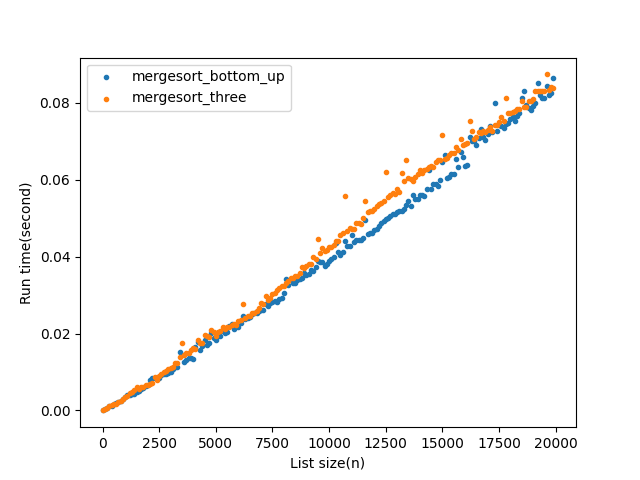
\includegraphics[width=0.49\textwidth]{Figures/mergesort_bottom_up_vs_mergesort_three.png}\label{r1}}
  \hfill
  \subfloat[Bottom\_up vs Three\_Top\_down \\  \centering{vs Three\_bottom\_up}]{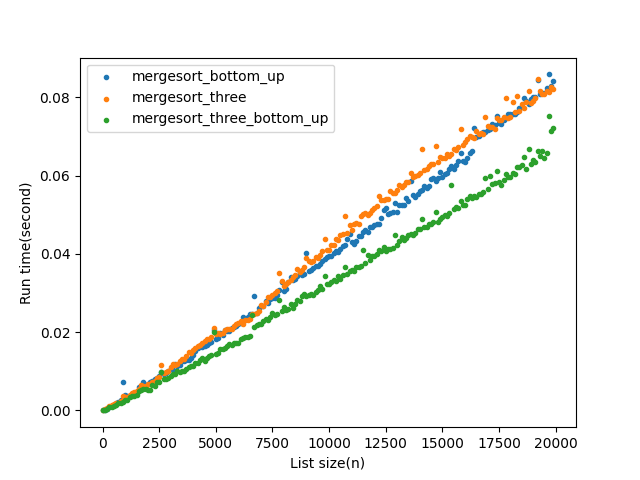
\includegraphics[width=0.49\textwidth]{Figures/mergesort_bottom_up_vs_mergesort_three_vs_mergesort_three_bottom_up.png}\label{r2}}
  \caption{Comparison for best algorithms}
\end{figure}

\newpage

\subsection{Best mergesort vs Factors(sorted)}
Under different sorted fators we obtained the average run times. 
We ran the algorithm 30 times with the length 20,000 list and took the 
average run time with different factors from 0.02 to 0.5, 
increasing the step of 0.02 each time. In Figure \ref{r3}, it seems to
be a linear function, but when we divide the run time with factor, 
 we can see that it is a power function, which is $0.0691x^{-0.99}$ 
 (Figure \ref{r5}).
It means that regarding sorted factors the 
\verb|mergesort_three_top_down| algorithm with the
fixed length of 20,000 has a time comlexity of $0.0691x^{0.01}$, 
which is a irrational function.

~\newline\noindent We interpreted it as due to the time
complexity of the comparison part of the algorithm. But the result was
slightly different from our expectation. Because we thought that
when a list is more sorted, it will increase the run time because
the relatively complicated comparison part of the algorithm will 
be implemented more frequently. 

~\newline\noindent However, as the time complexity of the algorithm
is $0.0691x^{0.01}$, which is extremly small, we can conclude that
the mergesort is not affacted by the sorted fatocrs. 
It means that the worst case time complexity of mergesort is
$O(nlogn)$.

\begin{figure}[hbt!]
  \centering
  \subfloat[Runtime \\ \centering{(n = 20,000, factor = 0 to 0.5)}]{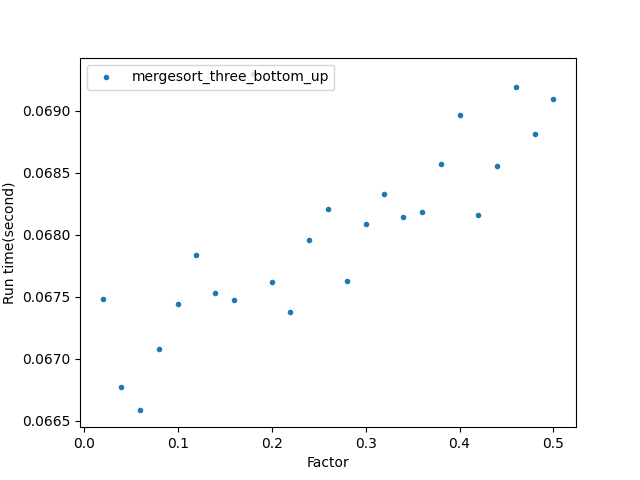
\includegraphics[width=0.49\textwidth]{Figures/mergesort_three_bottom_up_factor1.png}\label{r3}}
  \hfill
  \subfloat[Runtime/factor  \\ \centering{(n = 20,000, factor = 0 to 0.5)}]{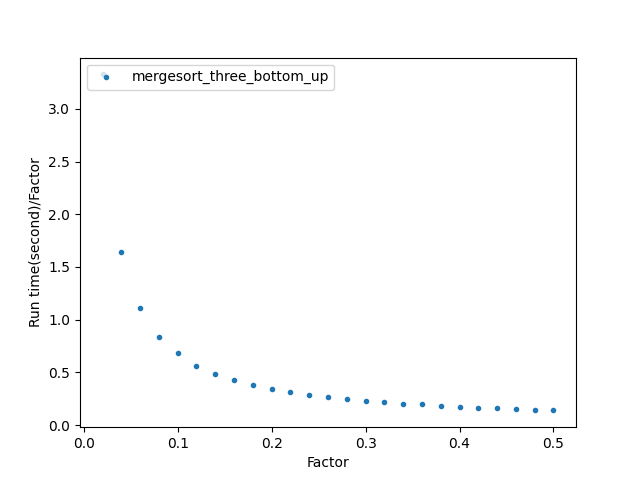
\includegraphics[width=0.49\textwidth]{Figures/mergesort_three_bottom_up_factor2.png}\label{r4}}
  \caption{Comparison under different sorted factors}
\end{figure}

\begin{figure}[hbt!]
  \centering
  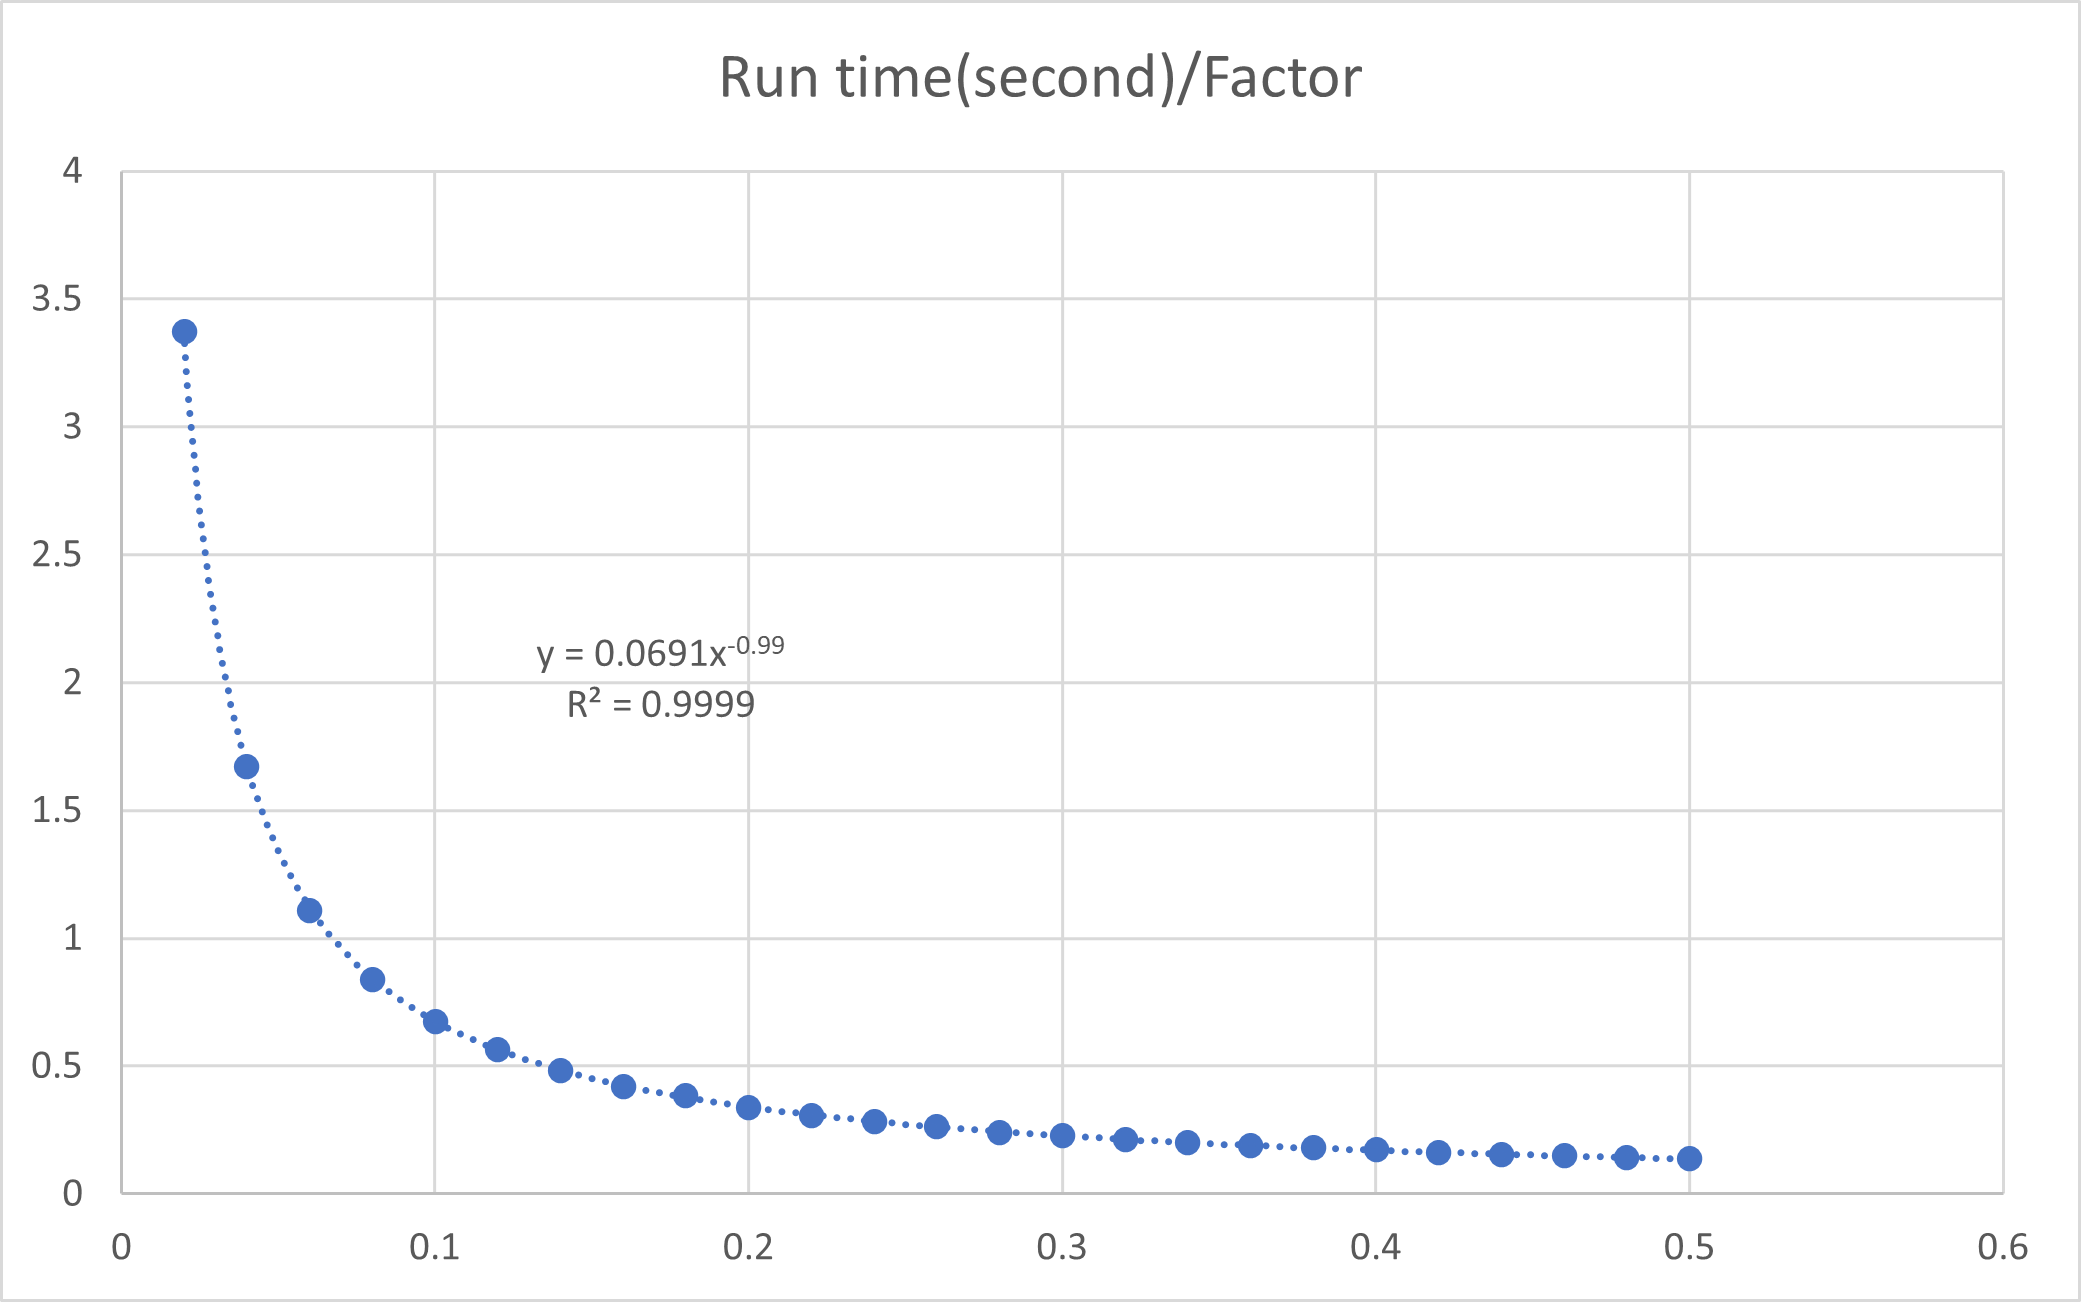
\includegraphics[width=0.5\textwidth,height=\textheight,keepaspectratio]{Figures/mergesort_three_bottom_up_sorted_factors.png}
  \caption{Runtime/factor  \\ \centering{(n = 20,000, factor = 0 to 0.5)}}
  \label{r5}
\end{figure}

\end{document}
